% Options for packages loaded elsewhere
% Options for packages loaded elsewhere
\PassOptionsToPackage{unicode}{hyperref}
\PassOptionsToPackage{hyphens}{url}
%
\documentclass[
  11pt,
  ignorenonframetext,
  aspectratio=169,
]{beamer}
\newif\ifbibliography
\usepackage{pgfpages}
\setbeamertemplate{caption}[numbered]
\setbeamertemplate{caption label separator}{: }
\setbeamercolor{caption name}{fg=normal text.fg}
\beamertemplatenavigationsymbolsempty
% remove section numbering
\setbeamertemplate{part page}{
  \centering
  \begin{beamercolorbox}[sep=16pt,center]{part title}
    \usebeamerfont{part title}\insertpart\par
  \end{beamercolorbox}
}
\setbeamertemplate{section page}{
  \centering
  \begin{beamercolorbox}[sep=12pt,center]{section title}
    \usebeamerfont{section title}\insertsection\par
  \end{beamercolorbox}
}
\setbeamertemplate{subsection page}{
  \centering
  \begin{beamercolorbox}[sep=8pt,center]{subsection title}
    \usebeamerfont{subsection title}\insertsubsection\par
  \end{beamercolorbox}
}
% Prevent slide breaks in the middle of a paragraph
\widowpenalties 1 10000
\raggedbottom
\AtBeginPart{
  \frame{\partpage}
}
\AtBeginSection{
  \ifbibliography
  \else
    \frame{\sectionpage}
  \fi
}
\AtBeginSubsection{
  \frame{\subsectionpage}
}
\usepackage{iftex}
\ifPDFTeX
  \usepackage[T1]{fontenc}
  \usepackage[utf8]{inputenc}
  \usepackage{textcomp} % provide euro and other symbols
\else % if luatex or xetex
  \usepackage{unicode-math} % this also loads fontspec
  \defaultfontfeatures{Scale=MatchLowercase}
  \defaultfontfeatures[\rmfamily]{Ligatures=TeX,Scale=1}
\fi
\usepackage{lmodern}

\ifPDFTeX\else
  % xetex/luatex font selection
\fi
% Use upquote if available, for straight quotes in verbatim environments
\IfFileExists{upquote.sty}{\usepackage{upquote}}{}
\IfFileExists{microtype.sty}{% use microtype if available
  \usepackage[]{microtype}
  \UseMicrotypeSet[protrusion]{basicmath} % disable protrusion for tt fonts
}{}
\makeatletter
\@ifundefined{KOMAClassName}{% if non-KOMA class
  \IfFileExists{parskip.sty}{%
    \usepackage{parskip}
  }{% else
    \setlength{\parindent}{0pt}
    \setlength{\parskip}{6pt plus 2pt minus 1pt}}
}{% if KOMA class
  \KOMAoptions{parskip=half}}
\makeatother

\usepackage{color}
\usepackage{fancyvrb}
\newcommand{\VerbBar}{|}
\newcommand{\VERB}{\Verb[commandchars=\\\{\}]}
\DefineVerbatimEnvironment{Highlighting}{Verbatim}{commandchars=\\\{\}}
% Add ',fontsize=\small' for more characters per line
\usepackage{framed}
\definecolor{shadecolor}{RGB}{241,243,245}
\newenvironment{Shaded}{\begin{snugshade}}{\end{snugshade}}
\newcommand{\AlertTok}[1]{\textcolor[rgb]{0.68,0.00,0.00}{#1}}
\newcommand{\AnnotationTok}[1]{\textcolor[rgb]{0.37,0.37,0.37}{#1}}
\newcommand{\AttributeTok}[1]{\textcolor[rgb]{0.40,0.45,0.13}{#1}}
\newcommand{\BaseNTok}[1]{\textcolor[rgb]{0.68,0.00,0.00}{#1}}
\newcommand{\BuiltInTok}[1]{\textcolor[rgb]{0.00,0.23,0.31}{#1}}
\newcommand{\CharTok}[1]{\textcolor[rgb]{0.13,0.47,0.30}{#1}}
\newcommand{\CommentTok}[1]{\textcolor[rgb]{0.37,0.37,0.37}{#1}}
\newcommand{\CommentVarTok}[1]{\textcolor[rgb]{0.37,0.37,0.37}{\textit{#1}}}
\newcommand{\ConstantTok}[1]{\textcolor[rgb]{0.56,0.35,0.01}{#1}}
\newcommand{\ControlFlowTok}[1]{\textcolor[rgb]{0.00,0.23,0.31}{\textbf{#1}}}
\newcommand{\DataTypeTok}[1]{\textcolor[rgb]{0.68,0.00,0.00}{#1}}
\newcommand{\DecValTok}[1]{\textcolor[rgb]{0.68,0.00,0.00}{#1}}
\newcommand{\DocumentationTok}[1]{\textcolor[rgb]{0.37,0.37,0.37}{\textit{#1}}}
\newcommand{\ErrorTok}[1]{\textcolor[rgb]{0.68,0.00,0.00}{#1}}
\newcommand{\ExtensionTok}[1]{\textcolor[rgb]{0.00,0.23,0.31}{#1}}
\newcommand{\FloatTok}[1]{\textcolor[rgb]{0.68,0.00,0.00}{#1}}
\newcommand{\FunctionTok}[1]{\textcolor[rgb]{0.28,0.35,0.67}{#1}}
\newcommand{\ImportTok}[1]{\textcolor[rgb]{0.00,0.46,0.62}{#1}}
\newcommand{\InformationTok}[1]{\textcolor[rgb]{0.37,0.37,0.37}{#1}}
\newcommand{\KeywordTok}[1]{\textcolor[rgb]{0.00,0.23,0.31}{\textbf{#1}}}
\newcommand{\NormalTok}[1]{\textcolor[rgb]{0.00,0.23,0.31}{#1}}
\newcommand{\OperatorTok}[1]{\textcolor[rgb]{0.37,0.37,0.37}{#1}}
\newcommand{\OtherTok}[1]{\textcolor[rgb]{0.00,0.23,0.31}{#1}}
\newcommand{\PreprocessorTok}[1]{\textcolor[rgb]{0.68,0.00,0.00}{#1}}
\newcommand{\RegionMarkerTok}[1]{\textcolor[rgb]{0.00,0.23,0.31}{#1}}
\newcommand{\SpecialCharTok}[1]{\textcolor[rgb]{0.37,0.37,0.37}{#1}}
\newcommand{\SpecialStringTok}[1]{\textcolor[rgb]{0.13,0.47,0.30}{#1}}
\newcommand{\StringTok}[1]{\textcolor[rgb]{0.13,0.47,0.30}{#1}}
\newcommand{\VariableTok}[1]{\textcolor[rgb]{0.07,0.07,0.07}{#1}}
\newcommand{\VerbatimStringTok}[1]{\textcolor[rgb]{0.13,0.47,0.30}{#1}}
\newcommand{\WarningTok}[1]{\textcolor[rgb]{0.37,0.37,0.37}{\textit{#1}}}

\usepackage{longtable,booktabs,array}
\newcounter{none} % for unnumbered tables
\usepackage{calc} % for calculating minipage widths
\usepackage{caption}
% Make caption package work with longtable
\makeatletter
\def\fnum@table{\tablename~\thetable}
\makeatother
\usepackage{graphicx}
\makeatletter
\newsavebox\pandoc@box
\newcommand*\pandocbounded[1]{% scales image to fit in text height/width
  \sbox\pandoc@box{#1}%
  \Gscale@div\@tempa{\textheight}{\dimexpr\ht\pandoc@box+\dp\pandoc@box\relax}%
  \Gscale@div\@tempb{\linewidth}{\wd\pandoc@box}%
  \ifdim\@tempb\p@<\@tempa\p@\let\@tempa\@tempb\fi% select the smaller of both
  \ifdim\@tempa\p@<\p@\scalebox{\@tempa}{\usebox\pandoc@box}%
  \else\usebox{\pandoc@box}%
  \fi%
}
% Set default figure placement to htbp
\def\fps@figure{htbp}
\makeatother





\setlength{\emergencystretch}{3em} % prevent overfull lines

\providecommand{\tightlist}{%
  \setlength{\itemsep}{0pt}\setlength{\parskip}{0pt}}



 


\setbeamertemplate{navigation symbols}{}
\setbeamertemplate{footline}[frame number]
\setbeamertemplate{itemize items}[circle]
\setbeamertemplate{itemize subitem}[triangle]
\setbeamercolor{frametitle}{fg=black}
\setbeamerfont{frametitle}{series=\bfseries}
\newcommand{\indep}{\perp\!\!\!\perp}
\usepackage{booktabs}
\usepackage{tikz}
\usetikzlibrary{arrows.meta,positioning,calc}
\tikzset{
  dnode/.style={circle,draw,thick,minimum size=9mm,inner sep=1pt,font=\small},
  unode/.style={circle,draw,thick,dashed,minimum size=9mm,inner sep=1pt,font=\small},
  bnode/.style={rectangle,draw,thick,fill=gray!25,minimum size=9mm,inner sep=3pt,font=\small},
  de/.style={-{Stealth[length=2.2mm]},thick},
  dde/.style={-{Stealth[length=2.2mm]},thick,dashed}
}
% shrink code input (fancyvrb) and code output (verbatim)
\usepackage{fancyvrb}
\fvset{fontsize=\scriptsize}
\makeatletter
\def\verbatim@font{\scriptsize\ttfamily}
\makeatother
\makeatletter
\@ifpackageloaded{caption}{}{\usepackage{caption}}
\AtBeginDocument{%
\ifdefined\contentsname
  \renewcommand*\contentsname{Table of contents}
\else
  \newcommand\contentsname{Table of contents}
\fi
\ifdefined\listfigurename
  \renewcommand*\listfigurename{List of Figures}
\else
  \newcommand\listfigurename{List of Figures}
\fi
\ifdefined\listtablename
  \renewcommand*\listtablename{List of Tables}
\else
  \newcommand\listtablename{List of Tables}
\fi
\ifdefined\figurename
  \renewcommand*\figurename{Figure}
\else
  \newcommand\figurename{Figure}
\fi
\ifdefined\tablename
  \renewcommand*\tablename{Table}
\else
  \newcommand\tablename{Table}
\fi
}
\@ifpackageloaded{float}{}{\usepackage{float}}
\floatstyle{ruled}
\@ifundefined{c@chapter}{\newfloat{codelisting}{h}{lop}}{\newfloat{codelisting}{h}{lop}[chapter]}
\floatname{codelisting}{Listing}
\newcommand*\listoflistings{\listof{codelisting}{List of Listings}}
\makeatother
\makeatletter
\makeatother
\makeatletter
\@ifpackageloaded{caption}{}{\usepackage{caption}}
\@ifpackageloaded{subcaption}{}{\usepackage{subcaption}}
\makeatother

\usepackage{bookmark}
\IfFileExists{xurl.sty}{\usepackage{xurl}}{} % add URL line breaks if available
\urlstyle{same}
\hypersetup{
  pdftitle={Unconfoundedness I: Assumptions and Matching},
  pdfauthor={Professor Ji-Woong Chung},
  hidelinks,
  pdfcreator={LaTeX via pandoc}}


\title{\texorpdfstring{Unconfoundedness I: Assumptions and
Matching}{Unconfoundedness I: Assumptions and Matching}}
\subtitle{\texorpdfstring{BUSS975: Causal Inference in Financial
Research}{BUSS975: Causal Inference in Financial Research}}
\author{Professor Ji-Woong Chung}
\date{}
\institute{Korea University}

\begin{document}
\frame{\titlepage}


\begin{frame}{Outline}
\protect\phantomsection\label{outline}
\begin{enumerate}
\tightlist
\item
  Introduction: what actually resolves bias
\item
  Confounders, covariates, and colliders
\item
  Identification assumptions
\item
  Subclassification
\item
  Exact matching
\item
  Nearest-neighbour matching
\item
  Inference with matching
\item
  Bias correction
\end{enumerate}

\vspace{0.6em}

Lecture 3b takes the same assumption and does something different with
it: collapse \(X\) to a single number, weight instead of match, and
compare all of it to regression.
\end{frame}

\section{1. Introduction}\label{introduction}

\begin{frame}{Where we left off}
\protect\phantomsection\label{where-we-left-off}
\begin{itemize}
\tightlist
\item
  Lecture 2 gave us a rule for \textbf{which} variables to condition on:
  block every backdoor path, condition on no descendant of \(D\).
\item
  It was silent on two things:

  \begin{itemize}
  \tightlist
  \item
    What if the variables that would close the backdoors are
    \textbf{unobserved}? (Usually the case.)
  \item
    Given a valid set, \textbf{how} do we actually condition --- and
    does it matter?
  \end{itemize}
\item
  This lecture takes the optimistic branch: \textbf{suppose the
  confounders are observed}. What then?
\item
  The methods --- subclassification, matching, propensity scores,
  regression --- are all answers to ``how.'' They differ less than their
  names suggest.
\end{itemize}
\end{frame}

\begin{frame}{Treatment assignment mechanisms resolve bias, not models}
\protect\phantomsection\label{treatment-assignment-mechanisms-resolve-bias-not-models}
Recall Lecture 1's decomposition. It is an \textbf{identity} --- true in
every dataset, experimental or not:

\[
\underbrace{E[Y|D{=}1] - E[Y|D{=}0]}_{SDO}
\;=\; ATE
\;+\; \underbrace{E[Y^0|D{=}1] - E[Y^0|D{=}0]}_{\text{selection on levels}}
\;+\; \underbrace{(1-\pi)(ATT - ATU)}_{\text{selection on gains}}
\]

\begin{itemize}
\tightlist
\item
  Nothing here is an assumption. The identity holds whatever you do.
\item
  \textbf{A regression cannot delete the last two terms.} No functional
  form, no set of fixed effects, no clustering choice touches them.
\item
  What deletes them is a \textbf{claim about how treatment was
  assigned}.
\end{itemize}
\end{frame}

\begin{frame}{What randomization actually did}
\protect\phantomsection\label{what-randomization-actually-did}
\begin{itemize}
\tightlist
\item
  Under \((Y^1,Y^0) \indep D\), we were permitted to \emph{deduce}: \[
  E[Y^0|D{=}1] = E[Y^0|D{=}0], \qquad E[Y^1|D{=}1] = E[Y^1|D{=}0]
  \]
\item
  The first kills selection on levels. Both together kill \(ATT - ATU\).
  What is left is the \(ATE\).
\item
  The deductions came from the \textbf{assignment mechanism}, not from
  any estimator. We then \emph{inserted} them into a statistical model.
\end{itemize}

\vspace{0.3em}
\begin{center}
\emph{The statistical model alone cannot resolve bias --- the statistical model matched with the assignment mechanism can.}
\end{center}
\end{frame}

\begin{frame}{Why this framing matters}
\protect\phantomsection\label{why-this-framing-matters}
\begin{itemize}
\tightlist
\item
  Randomization is an \textbf{assignment mechanism}, not a statistical
  model. A regression is a \textbf{statistical model}, not an assignment
  mechanism.
\item
  Confusing the two produces the most common error in empirical finance:
  believing that a long enough control list is itself an identification
  strategy.
\item
  Unconfoundedness is this lecture's assignment mechanism. It says
  treatment was assigned \textbf{as if at random within strata of
  \(X\)}.
\item
  Everything that follows --- subclassification, matching, propensity
  scores, regression --- is a statistical model that becomes credible
  \emph{only} if you can defend that mechanism.
\item
  So the order of business is: defend the mechanism first, choose the
  estimator second.
\end{itemize}
\end{frame}

\begin{frame}{The bet we are making}
\protect\phantomsection\label{the-bet-we-are-making}
\begin{center}
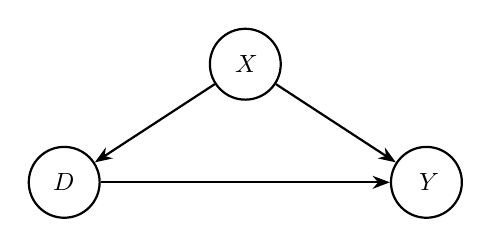
\begin{tikzpicture}
\node[dnode] (D) at (0,0)   {$D$};
\node[dnode] (Y) at (4.6,0) {$Y$};
\node[dnode] (X) at (2.3,1.5) {$X$};
\draw[de] (D) -- (Y);
\draw[de] (X) -- (D);
\draw[de] (X) -- (Y);
\end{tikzpicture}
\end{center}

\begin{itemize}
\tightlist
\item
  Everything rests on one claim: \textbf{there is no dashed circle}. No
  unobserved \(U\) pointing at both \(D\) and \(Y\).
\item
  That claim is \textbf{not testable}. No diagnostic, balance table, or
  specification test can establish it.
\item
  It is defended with institutional knowledge, not statistics --- which
  is why this lecture spends as much time on \emph{what could go wrong}
  as on estimators.
\item
  The literature calls it \textbf{unconfoundedness}, \textbf{conditional
  independence (CIA)}, or \textbf{selection on observables}. Same thing.
\end{itemize}
\end{frame}

\section{2. Confounders, Covariates, and
Colliders}\label{confounders-covariates-and-colliders}

\begin{frame}{A worked DAG: first class on the Titanic}
\protect\phantomsection\label{a-worked-dag-first-class-on-the-titanic}
\begin{itemize}
\tightlist
\item
  \textbf{Question}: did a first-class ticket (\(D\)) raise your chance
  of surviving (\(Y\))?
\item
  The raw comparison is stark: \(62.5\%\) of first-class passengers
  survived, versus \(27.1\%\) of everyone else --- a gap of \(35.4\)
  percentage points.
\item
  But the \emph{``women and children first''} rule was actually
  enforced, and first-class cabins were closer to the boat deck.
\item
  So \textbf{sex} and \textbf{age} drive both who bought a first-class
  ticket and who got into a lifeboat. Textbook confounding.
\item
  We use this because the data are real, complete, and small enough to
  compute by hand --- and because the confounders are not in dispute.
\end{itemize}
\end{frame}

\begin{frame}{The Titanic DAG}
\protect\phantomsection\label{the-titanic-dag}
\begin{center}
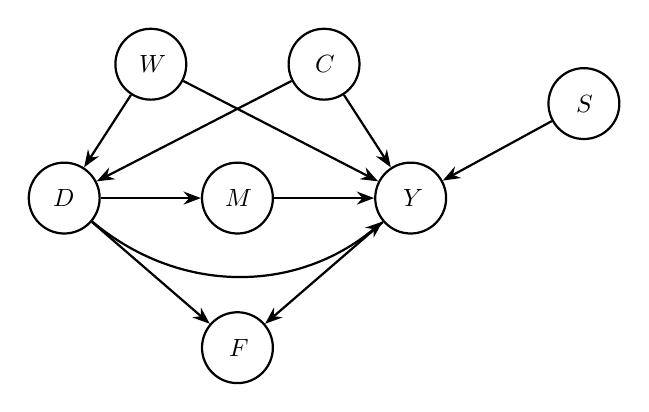
\begin{tikzpicture}
\node[dnode] (D) at (0,0)     {$D$};
\node[dnode] (M) at (2.2,0)   {$M$};
\node[dnode] (Y) at (4.4,0)   {$Y$};
\node[dnode] (W) at (1.1,1.7) {$W$};
\node[dnode] (C) at (3.3,1.7) {$C$};
\node[dnode] (F) at (2.2,-1.9){$F$};
\node[dnode] (S) at (6.6,1.2) {$S$};
\draw[de] (D) -- (M); \draw[de] (M) -- (Y);
\draw[de] (D) to[bend right=40] (Y);
\draw[de] (W) -- (D); \draw[de] (W) -- (Y);
\draw[de] (C) -- (D); \draw[de] (C) -- (Y);
\draw[de] (D) -- (F); \draw[de] (Y) -- (F);
\draw[de] (S) -- (Y);
\end{tikzpicture}
\end{center}

\vspace{-0.3em}

\footnotesize

\(D\) first class \quad \(Y\) survival \quad \(W\) sex \quad \(C\) age
\quad \(M\) lifeboat \quad \(F\) fame \quad \(S\) swimming

\normalsize

\begin{itemize}
\tightlist
\item
  Backdoor paths: \(D \leftarrow W \rightarrow Y\) and
  \(D \leftarrow C \rightarrow Y\). Both \textbf{open}. Condition on
  \(\{W,C\}\) and both close.
\item
  \(F\) is a \textbf{collider}: \(D \rightarrow F \leftarrow Y\).
  Already closed; conditioning on it \emph{opens} it.
\item
  \(M\) is a \textbf{mediator}: first class sat nearer the boat deck. It
  is \emph{part of} the effect, not a confounder of it.
\end{itemize}
\end{frame}

\begin{frame}{Four kinds of variable}
\protect\phantomsection\label{four-kinds-of-variable}
\begin{center}
\begin{tabular}{llp{6.5cm}}
\toprule
Type & Example & What conditioning does \\
\midrule
\textbf{Confounder}       & $W$ sex, $C$ age & \textbf{Required.} Closes a backdoor path. \\
\textbf{Collider}         & $F$ fame         & \textbf{Forbidden.} Opens a closed path. \\
\textbf{Neutral / precision} & $S$ swimming  & Optional. No bias either way; shrinks the standard error. \\
\textbf{Mediator}         & $M$ lifeboat    & \textbf{Forbidden} for the total effect. Blocks the causal path. \\
\bottomrule
\end{tabular}
\end{center}

\vspace{0.4em}

\begin{itemize}
\tightlist
\item
  Only one of these four rows is about bias \emph{reduction}. Two are
  about bias \emph{creation}.
\item
  Note \(S\): it predicts the outcome but not treatment. Free precision
  --- the honest case for controls that are not confounders.
\item
  \(M\) is the subtle one. Conditioning on it asks: \emph{did first
  class help, holding fixed the main way it helped?} Near zero --- and
  the wrong question.
\item
  The categories are properties of the \textbf{graph}, not the variable.
  Press coverage \emph{before} boarding would not be a collider.
\end{itemize}
\end{frame}

\begin{frame}{The same DAG in corporate finance}
\protect\phantomsection\label{the-same-dag-in-corporate-finance}
Effect of a \textbf{bank credit line} (\(D\)) on \textbf{firm
investment} (\(Y\)):

\begin{center}
\begin{tabular}{lll}
\toprule
Titanic & Finance analogue & Rule \\
\midrule
$W$, $C$ sex, age  & Firm size, industry, credit rating & Condition on \\
$F$ fame           & \emph{Subsequent} analyst coverage & Never condition on \\
$S$ swimming       & Pre-period export-market demand    & Optional, improves precision \\
$M$ lifeboat       & Amount actually drawn on the line  & Never condition on \\
--- & Unobserved managerial quality & The thing that sinks you \\
\bottomrule
\end{tabular}
\end{center}

\vspace{0.4em}

\begin{itemize}
\tightlist
\item
  Analyst coverage is the finance collider you will meet: it responds
  \emph{both} to the financing event and to firm performance.
\item
  The drawn amount is the mediator a referee will \emph{ask} you for ---
  ``surely control for how much they actually borrowed.'' That removes
  the channel you are trying to measure.
\item
  The last row has no Titanic counterpart, and that is the whole
  problem. On the Titanic we know the confounders are sex and age. In
  finance we rarely do.
\end{itemize}
\end{frame}

\begin{frame}{Covariate selection without a DAG}
\protect\phantomsection\label{covariate-selection-without-a-dag}
In practice you rarely have expert consensus on the full graph. Three
working rules:

\begin{enumerate}
\tightlist
\item
  \textbf{Include variables you are confident are confounders.} Prior
  knowledge about the assignment mechanism is the input, not the data.
\item
  \textbf{Include pre-treatment variables that strongly predict the
  outcome.} These are either confounders or precision-improvers like
  \(S\). Crucially, they are \emph{probably not colliders} --- a
  variable measured before treatment cannot be caused by it.
\item
  \textbf{Exclude anything that might be an outcome.} If you are unsure,
  exclude everything measured after treatment.
\end{enumerate}

\vspace{0.3em}

\begin{itemize}
\tightlist
\item
  Rule 2 does most of the work in practice, and rule 3 is the one most
  often violated in finance.
\item
  ``Pre-treatment'' is doing heavy lifting in rule 2. It is a timing
  argument, and timing is checkable.
\end{itemize}
\end{frame}

\section{3. Identification
Assumptions}\label{identification-assumptions}

\begin{frame}{Selecting the target parameter}
\protect\phantomsection\label{selecting-the-target-parameter}
Before estimating anything, decide \emph{whose} effect you want.

\[
ATE = E[Y^1 - Y^0], \quad
ATT = E[Y^1 - Y^0 \mid D{=}1], \quad
ATU = E[Y^1 - Y^0 \mid D{=}0]
\]

\begin{itemize}
\tightlist
\item
  Cunningham's example: a polio vaccine. The three parameters answer
  three different policy questions.

  \begin{itemize}
  \tightlist
  \item
    \(ATE\): what if we vaccinate \textbf{everyone}?
  \item
    \(ATT\): how much did the vaccine help \textbf{those who took it}?
  \item
    \(ATU\): what would happen if we reached \textbf{the currently
    unvaccinated}?
  \end{itemize}
\item
  These coincide only under constant treatment effects. With
  heterogeneity they differ, sometimes a lot.
\item
  \textbf{The estimand is a choice you make about the policy question.}
\end{itemize}
\end{frame}

\begin{frame}{Which parameter does the question need?}
\protect\phantomsection\label{which-parameter-does-the-question-need}
\begin{center}
\begin{tabular}{p{5.6cm}l}
\toprule
Finance question & Parameter \\
\midrule
Should the regulator extend this mandate to all firms? & $ATE$ \\
Did the firms that adopted IFRS benefit from it? & $ATT$ \\
Would forcing non-adopters to adopt help them? & $ATU$ \\
\bottomrule
\end{tabular}
\end{center}

\vspace{0.4em}

\begin{itemize}
\tightlist
\item
  Note the third row: it is the \emph{expansion} question, and it is
  almost never the one your data can answer well.
\item
  Papers routinely estimate the \(ATT\) and then write policy
  conclusions that require the \(ATE\) or \(ATU\). Watch for this in
  referee reports --- including your own.
\end{itemize}
\end{frame}

\begin{frame}{Unconfoundedness is a version of independence}
\protect\phantomsection\label{unconfoundedness-is-a-version-of-independence}
\begin{itemize}
\tightlist
\item
  \textbf{Strong unconfoundedness:} \[
  (Y^1, Y^0) \;\indep\; D \;\mid\; X
  \]
\item
  Compare Lecture 1's randomization assumption, \((Y^1,Y^0) \indep D\),
  with no conditioning.
\item
  In words: among units with the \emph{same} \(X\), treatment is as good
  as randomly assigned. It is \textbf{conditional randomization}.
\item
  This is the assignment mechanism from §1, Introduction, stratum by
  stratum: \[
  \begin{aligned}
  E[Y^1 \mid X{=}x] &= E[Y^1 \mid D{=}1, X{=}x] = E[Y^1 \mid D{=}0, X{=}x] \\[0.7em]
  E[Y^0 \mid X{=}x] &= E[Y^0 \mid D{=}1, X{=}x] = E[Y^0 \mid D{=}0, X{=}x]
  \end{aligned}
  \]
\item
  Strong because it's conditional independence with respect to
  \textbf{both} potential outcomes.
\end{itemize}
\end{frame}

\begin{frame}{What the assumption buys: plug-in}
\protect\phantomsection\label{what-the-assumption-buys-plug-in}
\begin{itemize}
\tightlist
\item
  The fundamental problem of causal inference is that \(Y^1\) and
  \(Y^0\) are never both observed.
\item
  Unconfoundedness lets us \textbf{replace a missing counterfactual with
  an observed outcome} from a comparable unit:
\end{itemize}

\[
\underbrace{E[Y^0 \mid D{=}1, X{=}x]}_{\text{never observed}}
\;=\;
\underbrace{E[Y^0 \mid D{=}0, X{=}x]}_{\text{observed}}
\;=\;
\underbrace{E[Y \mid D{=}0, X{=}x]}_{\text{in your data}}
\]

\begin{itemize}
\tightlist
\item
  The first equality is the \textbf{assumption}. The second is the
  switching equation --- pure definition.
\item
  Every method in this lecture is a different way of executing that
  substitution.
\item
  So switching estimators cannot rescue a design: all of them lean on
  the first equality, and none of them can test it.
  \textbf{Identification} credibility is common to all.
\item
  They \emph{do} differ downstream --- functional form, extrapolation
  into thin regions, which strata get weight. Those are
  \textbf{estimation} differences; Lecture 3b, §3, What Matching Cannot
  Do, returns to them.
\end{itemize}
\end{frame}

\begin{frame}{Unconfoundedness is controversial}
\protect\phantomsection\label{unconfoundedness-is-controversial}
\begin{itemize}
\tightlist
\item
  Read literally, the assumption says: firms with identical observables
  effectively \textbf{flip a coin} over a major financial decision.
\item
  Every model of optimizing behaviour says otherwise. Firms choose
  treatment \emph{because} they expect to benefit --- Lecture 1's
  selection on gains.
\item
  This is the deepest objection, and it comes from economics, not
  statistics.
\item
  It is not a reason never to use these methods. It is a reason to
  state, explicitly, why \emph{your} setting escapes it.
\end{itemize}
\end{frame}

\begin{frame}{Guido W. Imbens's three defences}
\protect\phantomsection\label{guido-w.-imbenss-three-defences}
\begin{enumerate}
\tightlist
\item
  \textbf{Statistical motivation.} It is the natural starting point.
\item
  \textbf{It is an empirical question.} With enough institutional
  knowledge, the relevant \(X\) may genuinely be measurable. Whether it
  is depends on the setting, not on econometrics.
\item
  \textbf{Objectives differ.} The decision-maker optimizes over
  something \emph{other than your outcome}. A firm choosing a credit
  line optimizes liquidity and covenant slack --- not the investment
  measure you happen to study.
\end{enumerate}

\vspace{0.3em}

\begin{itemize}
\tightlist
\item
  Defence 3 is the strongest available, and worth naming explicitly when
  you use it.
\item
  It also tells you when the design \emph{fails}: when the agent is
  optimizing over precisely your outcome variable.
\end{itemize}
\end{frame}

\begin{frame}{Road map: two routes through this chapter}
\protect\phantomsection\label{road-map-two-routes-through-this-chapter}
Everything ahead assumes unconfoundedness. The methods split on
\textbf{what they do when a treated unit has no comparable control.}

\begin{center}
\begin{tabular}{lp{4.3cm}p{4.3cm}}
\toprule
 & \textbf{Route 1: interpolation} & \textbf{Route 2: extrapolation} \\
\midrule
Rests on       & Common support & Functional form \\
Fills the gap by & It does not --- it refuses & Projecting the fitted model into it \\
Methods        & Subclassification, matching, propensity scores & Regression \\
Covered in     & §4--§8, and Lecture 3b §1 & Lecture 3b §2 \\
\bottomrule
\end{tabular}
\end{center}
\end{frame}

\begin{frame}{Common support}
\protect\phantomsection\label{common-support}
\begin{itemize}
\tightlist
\item
  Unconfoundedness alone is not enough. You also need units to compare.
\item
  \textbf{Strong common support} (needed for the \(ATE\)): \[
  0 < \Pr(D=1 \mid X = x) < 1 \quad \text{for all } x
  \] At every value of \(X\), both treated and untreated units must
  exist. \textless!-- - Cunningham's jigsaw analogy:
  \textbf{unconfoundedness is the blueprint; common support is whether
  the pieces are actually in the box.}
\item
  A perfect blueprint is useless if a piece is missing --- and a
  complete box is useless if the blueprint is wrong. --\textgreater{}
\end{itemize}
\end{frame}

\begin{frame}{The two assumptions differ in kind}
\protect\phantomsection\label{the-two-assumptions-differ-in-kind}
\begin{center}
\begin{tabular}{ll}
\toprule
\textbf{Unconfoundedness} & \textbf{Common support} \\
\midrule
Untestable & \textbf{Verifiable in your data} \\
Defended with institutional knowledge & Checked with a histogram \\
Failure $\Rightarrow$ bias & Failure $\Rightarrow$ extrapolation \\
\bottomrule
\end{tabular}
\end{center}

\vspace{0.4em}

\begin{itemize}
\tightlist
\item
  You can have one without the other, and the failures look nothing
  alike.
\item
  Common support is the assumption you have \textbf{no excuse} for not
  checking --- and the one most papers skip.
\item
  This distinction is the key to the NSW debate at the end of this
  lecture.
\end{itemize}
\end{frame}

\begin{frame}{Weighting treatment effects under unconfoundedness}
\protect\phantomsection\label{weighting-treatment-effects-under-unconfoundedness}
Put the two assumptions together and the \(ATE\) becomes computable.

\[
\begin{aligned}
ATE(x) &= E\big[\,Y^1 \mid X{=}x\,\big] - E\big[\,Y^0 \mid X{=}x\,\big] \\
       &= \underbrace{E\big[\,Y^1 \mid D{=}1, X{=}x\,\big] - E\big[\,Y^0 \mid D{=}0, X{=}x\,\big]}_{\text{unconfoundedness --- used on \emph{both} terms}} \\
       &= \underbrace{E\big[\,Y \mid D{=}1, X{=}x\,\big] - E\big[\,Y \mid D{=}0, X{=}x\,\big]}_{\text{switching equation}} \\[0.3em]
ATE    &= \underbrace{\sum_x \Big( E[Y \mid D{=}1, X{=}x] - E[Y \mid D{=}0, X{=}x] \Big)\Pr(X{=}x)}_{\text{iterated expectations; common support}}
\end{aligned}
\]

\begin{itemize}
\tightlist
\item
  \(ATE(x)\) is the effect \textbf{within stratum \(x\)} ---
  \emph{conditional average treatment effect} (CATE). The last line
  averages those with \textbf{population} weights.
\item
  \textbf{Unconfoundedness is used twice}, once for \(Y^1\) and once for
  \(Y^0\). That is precisely why the \(ATE\) needs the \emph{strong}
  version.
\end{itemize}
\end{frame}

\begin{frame}{A three-stratum example}
\protect\phantomsection\label{a-three-stratum-example}
Suppose the effect on mortality differs by age group, and the groups are
equally sized:

\begin{center}
\begin{tabular}{lcc}
\toprule
Stratum & Effect in stratum (pp) & $\Pr(X = x)$ \\
\midrule
Young       & $80$  & $1/3$ \\
Middle-aged & $55$  & $1/3$ \\
Old         & $100$ & $1/3$ \\
\bottomrule
\end{tabular}
\end{center}

\[
\begin{aligned}
  \widehat{\mathit{ATE}} &= \frac{N_y}{N} \times SDO_{y} +
  \frac{N_m}{N} \times SDO_{m} + \frac{N_o}{N} \times SDO_{o} \\
  &= \frac{1}{3} \times 80 + \frac{1}{3} \times 55 + \frac{1}{3} \times 100 \\
  &= 78.33
\end{aligned}
\]

\begin{itemize}
\tightlist
\item
  The \(ATE\) is a number \textbf{no stratum experiences}. It describes
  a population, not a unit.
\end{itemize}
\end{frame}

\begin{frame}{Estimating the ATT under weaker assumptions}
\protect\phantomsection\label{estimating-the-att-under-weaker-assumptions}
\begin{itemize}
\tightlist
\item
  A weaker assumption suffices if you only want the \(ATT\): \[
  Y^0 \;\indep\; D \;\mid\; X
  \]
\item
  Only the \textbf{untreated} potential outcome must be independent of
  treatment.
\item
  It allows firms to \emph{anticipate their own gains} \(Y^1\) and
  select on them, while assuming they do not select on how they would
  have done anyway.

  \begin{itemize}
  \tightlist
  \item
    In finance that ordering is often defensible. A firm knows its
    expected benefit from a credit line better than it knows its
    counterfactual path without one.
  \end{itemize}
\item
  \textbf{Weak common support}: Controls must exist wherever treated
  units do --- but not conversely. \[
  \Pr(D = 0 \mid X) > 0 \quad \text{for all } X \text{ such that }
  \Pr(D = 1 \mid X) > 0 
  \]
\end{itemize}
\end{frame}

\begin{frame}{Why the asymmetry makes sense}
\protect\phantomsection\label{why-the-asymmetry-makes-sense}
\[
\begin{aligned}
ATT(x) &= E[Y^1 \mid D{=}1, X{=}x] - E[Y^0 \mid D{=}1, X{=}x] \\[0.3em]
       &= \underbrace{E[Y \mid D{=}1, X{=}x]}_{\text{switching equation}} - E[Y^0 \mid D{=}1, X{=}x] \\[0.3em]
       &= E[Y \mid D{=}1, X{=}x] - \underbrace{E[Y \mid D{=}0, X{=}x]}_{\text{weak unconfoundedness}} \\[0.4em]
ATT    &= \underbrace{\sum_x \Big( E[Y \mid D{=}1, X{=}x] - E[Y \mid D{=}0, X{=}x] \Big)\Pr(X{=}x \mid D{=}1)}_{\text{common support, wherever treated units live}}
\end{aligned}
\]

\begin{itemize}
\tightlist
\item
  Weighting by \(\Pr(X \mid D{=}1)\) --- covariates \textbf{among the
  treated} --- is what makes it the \(ATT\): strata with no treated
  units get zero weight.
\item
  \textbf{Rule}: if you can only defend the weak version, your estimand
  is the \(ATT\). Say so.
\end{itemize}
\end{frame}

\section{4. Subclassification}\label{subclassification}

\begin{frame}{Cochran's method}
\protect\phantomsection\label{cochrans-method}
\begin{itemize}
\tightlist
\item
  The oldest estimator here, and the most transparent. Three steps:

  \begin{enumerate}
  \tightlist
  \item
    \textbf{Stratify} on \(X\).
  \item
    Compute the treated-minus-control difference \textbf{within} each
    stratum.
  \item
    \textbf{Average} the strata, weighting by whatever the estimand
    requires.
  \end{enumerate}
\item
  No functional form is assumed. Within a stratum, units are identical
  on \(X\) by construction.
\item
  The weights define the estimand:
\end{itemize}

\begin{center}
\begin{tabular}{lll}
\toprule
Estimand & Weight stratum $k$ by & Interpretation \\
\midrule
$ATE$ & $n_k / N$                      & population share \\
$ATT$ & $n_{k,\text{treated}} / N_{\text{treated}}$   & treated share \\
$ATU$ & $n_{k,\text{untreated}} / N_{\text{untreated}}$ & control share \\
\bottomrule
\end{tabular}
\end{center}
\end{frame}

\begin{frame}{The Titanic: the raw comparison}
\protect\phantomsection\label{the-titanic-the-raw-comparison}
\begin{itemize}
\tightlist
\item
  Treated: 325 first-class passengers, \(62.5\%\) survived.
\item
  Control: 1,876 others, \(27.1\%\) survived. \[
  SDO = 62.5 - 27.1 = 35.4 \text{ percentage points}
  \]
\item
  Taken at face value: a first-class ticket nearly \emph{tripled} your
  survival odds.
\item
  But the first-class cabins held a very different mix of people. Sex
  and age are confounders, and we can see them directly.
\item
  Stratify on \(\{\)sex, age\(\}\): four strata, and every one of them
  is occupied.
\end{itemize}
\end{frame}

\begin{frame}{The four strata}
\protect\phantomsection\label{the-four-strata}
\begin{center}
\begin{tabular}{lrrrrr}
\toprule
Stratum & $n$ & first class & survival, 1st & survival, other & difference \\
\midrule
Adult male   & 1,667 & 175 & $32.6\%$  & $18.8\%$ & $13.7$ pp \\
Adult female &   425 & 144 & $97.2\%$  & $62.6\%$ & $34.6$ pp \\
Male child   &    64 &   5 & $100.0\%$ & $40.7\%$ & $59.3$ pp \\
Female child &    45 &   1 & $100.0\%$ & $61.4\%$ & $38.6$ pp \\
\bottomrule
\end{tabular}
\end{center}

\vspace{0.4em}

\begin{itemize}
\tightlist
\item
  Every within-stratum difference is \textbf{smaller than the \(35.4\)
  pp raw gap.} Confounding was inflating the estimate.
\item
  Look at the composition: \(76\%\) of all passengers were adult males
  --- the stratum with the \emph{smallest} effect --- but only \(54\%\)
  of first class.
\item
  Note the last stratum: \textbf{one} first-class female child. Remember
  her; she returns shortly.
\end{itemize}
\end{frame}

\begin{frame}{Three estimands, three answers}
\protect\phantomsection\label{three-estimands-three-answers}
Same four differences. Only the weights change.

\begin{center}
\begin{tabular}{lrrrr}
\toprule
Weight on & Adult male & Adult female & Male child & Female child \\
\midrule
$ATE$ (population share)  & $0.757$ & $0.193$ & $0.029$ & $0.020$ \\
$ATT$ (treated share)     & $0.538$ & $0.443$ & $0.015$ & $0.003$ \\
$ATU$ (control share)     & $0.795$ & $0.150$ & $0.031$ & $0.023$ \\
\bottomrule
\end{tabular}
\end{center}

\vspace{0.3em}

\[
\widehat{ATE} = 19.6 \text{ pp}, \qquad
\widehat{ATT} = 23.8 \text{ pp}, \qquad
\widehat{ATU} = 18.9 \text{ pp}
\]

\begin{itemize}
\tightlist
\item
  The raw \(35.4\) pp falls to roughly \textbf{20 pp} once composition
  is held fixed. Nearly half the headline gap was confounding.
\item
  \(ATT > ATE\) because first class was disproportionately adult
  \emph{female} --- the stratum with a large effect.
\end{itemize}
\end{frame}

\begin{frame}{The curse of dimensionality}
\protect\phantomsection\label{the-curse-of-dimensionality}
\begin{itemize}
\tightlist
\item
  Now delete one passenger: the single first-class female child.
\item
  That stratum still exists --- 44 girls travelled in other classes ---
  but it now has \textbf{no treated unit}. The within-stratum difference
  is undefined.
\end{itemize}

\begin{center}
\begin{tabular}{lc}
\toprule
Parameter & Still identified? \\
\midrule
$ATE$ & \textbf{No} --- needs all four differences \\
$ATU$ & \textbf{No} --- female children get weight $0.023$ \\
$ATT$ & \textbf{Yes} --- $23.7$ pp from the three occupied strata \\
\bottomrule
\end{tabular}
\end{center}

\vspace{0.4em}

\begin{itemize}
\tightlist
\item
  One passenger out of 2,201 destroys two of the three parameters. The
  \(ATT\) survives because it never needed that cell.
\item
  This is common support failing.
\end{itemize}
\end{frame}

\begin{frame}{Why it gets worse fast}
\protect\phantomsection\label{why-it-gets-worse-fast}
\begin{itemize}
\tightlist
\item
  One binary covariate: 2 strata. Ten binary covariates:
  \(2^{10} = 1{,}024\). One continuous covariate: infinitely many.
\item
  Cells multiply exponentially; your sample does not. Empty cells become
  the norm, not the exception.
\item
  Non-parametric methods --- subclassification, exact matching,
  reweighting --- \textbf{break down honestly}: they simply cannot
  compute the estimate.
\item
  Regression \textbf{does not break down}. It extrapolates across the
  empty cells using functional form, and reports a number with a
  standard error.
\end{itemize}
\end{frame}

\section{5. Exact Matching}\label{exact-matching}

\begin{frame}{Matching as explicit imputation}
\protect\phantomsection\label{matching-as-explicit-imputation}
\begin{itemize}
\tightlist
\item
  Every causal inference is an imputation problem: the counterfactual is
  missing and must be filled in.
\item
  Most methods impute \textbf{implicitly}, inside a formula. Matching
  does it \textbf{explicitly}, unit by unit --- and that transparency is
  its main virtue.
\item
  Start from the definition of the \(ATT\). Exactly \textbf{one} term is
  unavailable:
\end{itemize}

\[
ATT \;=\; \underbrace{E[Y^1 \mid D{=}1]}_{\text{observed: } Y = Y^1 \text{ when } D=1}
\;-\; \underbrace{E[Y^0 \mid D{=}1]}_{\textbf{missing}}
\]

\begin{itemize}
\tightlist
\item
  The first term is just the treated sample mean. Everything matching
  does is build a stand-in for the second.
\end{itemize}
\end{frame}

\begin{frame}{Replacing the missing term}
\protect\phantomsection\label{replacing-the-missing-term}
Condition on \(X\), and the assumption does its work:

\[
\begin{aligned}
E[Y^0 \mid D{=}1, X{=}x]
  &= \underbrace{E[Y^0 \mid D{=}0, X{=}x]}_{\text{weak unconfoundedness}} \\[0.2em]
  &= \underbrace{E[Y \mid D{=}0, X{=}x]}_{\text{switching equation}} \\[0.4em]
E[Y^0 \mid D{=}1]
  &= \underbrace{\sum_x E[Y \mid D{=}0, X{=}x]\,\Pr(X{=}x \mid D{=}1)}_{\text{common support: this must exist wherever treated units live}}
\end{aligned}
\]

\begin{itemize}
\tightlist
\item
  The missing quantity is now written entirely in terms of things you
  can estimate from control units.
\item
  \textbf{Matching is simply a non-parametric estimate of
  \(E[Y \mid D{=}0, X{=}X_i]\)} --- take the controls that look like
  \(i\), and average them.
\end{itemize}
\end{frame}

\begin{frame}{The estimator, and what to do about ties}
\protect\phantomsection\label{the-estimator-and-what-to-do-about-ties}
Let \(\mathcal{J}(i)\) be the set of control units matched to treated
unit \(i\), and \(M_i = |\mathcal{J}(i)|\).

\[
\widehat{ATT} \;=\; \frac{1}{N_T}\sum_{i\,:\,D_i = 1}
\Bigg( Y_i - \underbrace{\frac{1}{M_i}\sum_{j \in \mathcal{J}(i)} Y_j}_{\widehat{Y^0_i}} \Bigg)
\]

\begin{itemize}
\tightlist
\item
  If two controls sit at exactly the same distance from \(i\), use both
  --- breaking the tie arbitrarily injects the analyst's coin flip into
  the estimate. \textless!-- - \(M_i\) also varies when a caliper binds:
  a treated unit with no control inside the caliper contributes nothing,
  and \(N_T\) must then count only the units you actually matched.
\item
  You can \emph{point at the specific firms} doing the work for each
  observation. No regression output permits that. --\textgreater{}
\end{itemize}
\end{frame}

\begin{frame}{The same idea for the ATE}
\protect\phantomsection\label{the-same-idea-for-the-ate}
For a control unit \(j\), the missing half is \(Y^1\). Let
\(\mathcal{I}(j)\) be the treated units matched to it,
\(M_j = |\mathcal{I}(j)|\).

\[
\widehat{ATE} = \frac{1}{N}\Bigg[
\underbrace{\sum_{i\,:\,D_i=1}\Big( Y_i - \tfrac{1}{M_i}\!\!\sum_{j \in \mathcal{J}(i)}\!\! Y_j \Big)}_{\text{treated: observed} \,-\, \text{imputed}}
\;+\;
\underbrace{\sum_{j\,:\,D_j=0}\Big( \tfrac{1}{M_j}\!\!\sum_{i \in \mathcal{I}(j)}\!\! Y_i - Y_j \Big)}_{\text{control: imputed} \,-\, \text{observed}}
\Bigg]
\]

\begin{itemize}
\tightlist
\item
  Every unit contributes one \emph{estimated} treatment effect; the
  \(ATE\) averages all \(N\) of them.
\item
  Equivalently
  \(\widehat{ATE} = \frac{N_T}{N}\widehat{ATT} + \frac{N_C}{N}\widehat{ATU}\)
  --- the weights from §4, Subclassification, back again.
\end{itemize}
\end{frame}

\begin{frame}{Exact matching and its limit}
\protect\phantomsection\label{exact-matching-and-its-limit}
\begin{itemize}
\tightlist
\item
  With discrete \(X\) and full common support, exact matching and
  subclassification give the \textbf{same answer}. They are the same
  estimator, organized differently.
\item
  The difference is bookkeeping: subclassification aggregates to stratum
  effects first; matching imputes unit by unit.
\item
  Same fatal problem, too: with a continuous covariate, \textbf{exact
  matches occur with probability zero.}
\item
  Two responses, and they define the next two sections:

  \begin{itemize}
  \tightlist
  \item
    Give up on exact equality --- match to the \emph{nearest} unit (§6,
    Nearest-Neighbour Matching), then correct that error (§8, Bias
    Correction).
  \item
    Give up on matching \(X\) itself --- match on a \emph{summary} of
    \(X\) (Lecture 3b, §1, Propensity Scores).
  \end{itemize}
\end{itemize}
\end{frame}

\section{6. Nearest-Neighbour
Matching}\label{nearest-neighbour-matching}

\begin{frame}{One confounder}
\protect\phantomsection\label{one-confounder}
\begin{itemize}
\tightlist
\item
  Drop the demand for exact equality. Match each treated unit to the
  control that minimizes \(|X_i - X_j|\).
\item
  The gap you accept is called the \textbf{matching discrepancy}, and
  §8, Bias Correction, is entirely about what it costs you.
\item
  Choices you must make and report:

  \begin{itemize}
  \tightlist
  \item
    \textbf{With or without replacement.} With replacement always takes
    the closest match, so it \textbf{lowers bias} and raises
    \textbf{variance.}
  \item
    \textbf{How many neighbours, \(M\).} More neighbours: less variance,
    more bias.
  \item
    \textbf{Caliper}: refuse any match beyond a maximum distance. Better
    to drop a treated unit than to match it to something unlike it.
  \end{itemize}
\end{itemize}
\end{frame}

\begin{frame}{Multiple dimensions and the distance metric}
\protect\phantomsection\label{multiple-dimensions-and-the-distance-metric}
With several covariates, ``closest'' requires a definition --- and the
choice changes the answer.

\begin{itemize}
\tightlist
\item
  \textbf{Euclidean}: \(\sqrt{\sum_k (X_{ik}-X_{jk})^2}\).
  Scale-dependent: a variable in won swamps one measured as a ratio.
\item
  \textbf{Normalized Euclidean}: divide each covariate by its standard
  deviation. Fixes scale, ignores correlation.
\item
  \textbf{Mahalanobis}: \(\sqrt{(X_i - X_j)' \Sigma^{-1}(X_i-X_j)}\).
  Standardizes scale \textbf{and} accounts for correlation between
  covariates. The default choice.
\end{itemize}

\vspace{0.3em}

\begin{itemize}
\tightlist
\item
  Why correlation matters: if size and leverage are highly correlated,
  Euclidean distance double-counts what is essentially one dimension.
\end{itemize}
\end{frame}

\section{7. Inference with Matching}\label{inference-with-matching}

\begin{frame}{Why the usual standard errors fail}
\protect\phantomsection\label{why-the-usual-standard-errors-fail}
\begin{itemize}
\tightlist
\item
  Matched observations are \textbf{dependent by construction}: the same
  control may serve several treated units, and the matches were chosen
  \emph{using the data}.
\item
  Conventional standard errors treat the matched sample as if it were
  drawn at random. It was not, and they understate uncertainty.
\item
  Abadie and Imbens (2008) show conventional standard errors is invalid
  for matching estimators
\item
  Use the \textbf{Abadie--Imbens variance estimator}, which prices in
  how many times each control was reused.
\item
  Practical note: check what your software reports \emph{by default}.
  Several packages report the naive standard error unless told
  otherwise.
\end{itemize}
\end{frame}

\begin{frame}{The Abadie--Imbens variance estimator}
\protect\phantomsection\label{the-abadieimbens-variance-estimator}
Let \(\hat\tau_i = Y_i - \frac{1}{M}\sum_{m=1}^{M} Y_{j_m(i)}\) be unit
\(i\)'s \textbf{own} effect, so
\(\widehat{ATT} = \frac{1}{N_T}\sum_{i:D_i=1}\hat\tau_i\) is their
average. \(K_j\) counts how often control \(j\) is used.

\[
\hat\sigma^2_{ATT} \;=\;
\underbrace{\frac{1}{N_T}\sum_{i\,:\,D_i=1}\big(\hat\tau_i - \widehat{ATT}\big)^2}_{\text{(a) spread of the unit-level effects}}
\;+\;
\underbrace{\frac{1}{N_T}\sum_{j\,:\,D_j=0}\frac{K_j(K_j-1)}{M^2}\,\hat\sigma^2(X_j)}_{\text{(b) penalty for reusing controls}}
\]

\[
\mathrm{SE}\big(\widehat{ATT}\big) \;=\; \sqrt{\hat\sigma^2_{ATT} \,\big/\, N_T}
\]

\begin{itemize}
\tightlist
\item
  So term (a) is simply the \textbf{sample variance of the
  \(\hat\tau_i\)}. Alone, it is the without-replacement formula: with
  \(K_j \in \{0,1\}\) term (b) vanishes.
\item
  \(\hat\sigma^2(X_j) = \mathrm{var}(Y \mid X_j, D{=}0)\), the outcome
  variance among controls.
\item
  Here \(M\) is \textbf{fixed} --- the clean \(K_j(K_j{-}1)\) split
  needs it.
\end{itemize}
\end{frame}

\begin{frame}[fragile]{In Stata}
\protect\phantomsection\label{in-stata}
Cunningham's training data: 10 trainees, 20 non-trainees, matched on
\texttt{age} and \texttt{gpa}.

\footnotesize

\begin{Shaded}
\begin{Highlighting}[]
\KeywordTok{use}\NormalTok{ https:}\CommentTok{//github.com/scunning1975/mixtape/raw/master/training\_inexact.dta, clear}

\NormalTok{* Minimized euclidean distance with usual }\KeywordTok{variance}\NormalTok{ and }\KeywordTok{robust}
\NormalTok{teffects nnmatch (earnings age gpa) (treat), atet nn(1) metric(eucl) }\KeywordTok{vce}\NormalTok{(iid)}
\NormalTok{teffects nnmatch (earnings age gpa) (treat), atet nn(1) metric(eucl) }\KeywordTok{generate}\NormalTok{(match1)}

\NormalTok{* Minimized Mahalanobis distance with usual }\KeywordTok{variance}\NormalTok{ and }\KeywordTok{robust}
\NormalTok{teffects nnmatch (earnings age gpa) (treat), atet nn(1) metric(maha) }\KeywordTok{vce}\NormalTok{(iid)}
\NormalTok{teffects nnmatch (earnings age gpa) (treat), atet nn(1) metric(maha) }\KeywordTok{generate}\NormalTok{(match2)}
\end{Highlighting}
\end{Shaded}

\normalsize

\begin{itemize}
\tightlist
\item
  \texttt{(earnings\ age\ gpa)} is outcome-then-covariates;
  \texttt{(treat)} is the treatment. \texttt{atet} asks for the \(ATT\),
  \texttt{nn(1)} for one neighbour.
\item
  \texttt{vce(iid)} is the constant-variance standard error.
  \textbf{Drop it and you get Abadie--Imbens} --- that is Stata's
  default, so the second command of each pair is the one to report.
\item
  \texttt{generate(match1)} writes each unit's matched partner back into
  the data. Always look at it.
\end{itemize}
\end{frame}

\begin{frame}[fragile]{Two metrics, two answers}
\protect\phantomsection\label{two-metrics-two-answers}
\begin{center}
\small
\begin{tabular}{lcccc}
\toprule
 & $\widehat{ATT}$ & \texttt{vce(iid)} & \textbf{Abadie--Imbens} & distinct controls used \\
\midrule
Euclidean    & $1607.5$ & $38.7$  & $38.7$  & 10 of 20 \\
Mahalanobis  & $1315.0$ & $325.5$ & $590.1$ & \textbf{3} of 20 \\
\midrule
\emph{Truth} & $1607.5$ & & & \\
\bottomrule
\end{tabular}
\end{center}

\begin{itemize}
\tightlist
\item
  \texttt{age} has standard deviation \(9.1\) and \texttt{gpa} only
  \(0.57\), so raw Euclidean distance is \textbf{matching on age and
  ignoring gpa} --- the scale problem from §6, Nearest-Neighbour
  Matching. Every trainee gets a \emph{different} control:
  \(K_j \leq 1\), term (b) is zero, both standard errors coincide.
\item
  Mahalanobis makes \texttt{gpa} count --- and \texttt{gpa} is noise.
  \textbf{Three controls end up serving all ten trainees}; one is used
  five times.
\item
  Term (a) alone still reports \(199.8\). The reuse correction triples
  it.
\end{itemize}
\end{frame}

\section{8. Bias Correction}\label{bias-correction}

\begin{frame}{The matching discrepancy is bias, not noise}
\protect\phantomsection\label{the-matching-discrepancy-is-bias-not-noise}
Matching was only \emph{approximate}: \(X_{j(i)} \approx X_i\), never
\(=\). What does the leftover gap cost?

\begin{itemize}
\tightlist
\item
  Abadie--Imbens (2006): More data does not help much.
\end{itemize}

\begin{itemize}
\tightlist
\item
  Usually you cannot get more data anyway. Abadie--Imbens (2011) is the
  second-best answer: \textbf{model the bias and subtract it.}
\end{itemize}
\end{frame}

\begin{frame}{An outcome model for the missing \(Y^0\)}
\protect\phantomsection\label{an-outcome-model-for-the-missing-y0}
\[
\begin{aligned}
\mu^0(x) &= E\big[\,Y \mid X{=}x, D{=}0\,\big] \;=\; \underbrace{E\big[\,Y^0 \mid X{=}x\,\big]}_{\text{unconfoundedness}} \\
\mu^1(x) &= E\big[\,Y \mid X{=}x, D{=}1\,\big] \;=\; \underbrace{E\big[\,Y^1 \mid X{=}x\,\big]}_{\text{unconfoundedness}} \\[0.3em]
Y_i &= \mu^{D_i}(X_i) + \varepsilon_i, \qquad E\big[\,\varepsilon_i \mid X_i, D_i\,\big] = 0
\end{aligned}
\]

\begin{itemize}
\tightlist
\item
  The second equality on each line \textbf{is} unconfoundedness. It is
  what lets a regression fitted on controls speak about treated units.
\item
  So far, all definition. The \textbf{assumption} arrives only when we
  choose a functional form for \(\hat\mu^0\).
\end{itemize}
\end{frame}

\begin{frame}{Where the bias hides}
\protect\phantomsection\label{where-the-bias-hides}
Substitute \(Y_i = \mu^{D_i}(X_i)+\varepsilon_i\) into
\(\widehat{ATT}=\frac{1}{N_T}\sum_{D_i=1}(Y_i - Y_{j(i)})\), subtract
the true \(ATT\), then add and subtract
\(\frac{1}{N_T}\sum_{D_i=1}\mu^0(X_i)\):

\[
\begin{aligned}
\widehat{ATT} - ATT \;=\;& \underbrace{\tfrac{1}{N_T}\textstyle\sum_{D_i=1}\big(\mu^1(X_i) - \mu^0(X_i) - ATT\big)}_{\text{(1) sampling variation in \emph{which} units got treated}} \\
+\;& \underbrace{\tfrac{1}{N_T}\textstyle\sum_{D_i=1}\big(\varepsilon_i - \varepsilon_{j(i)}\big)}_{\text{(2) mean-zero noise}} \\
+\;& \underbrace{\tfrac{1}{N_T}\textstyle\sum_{D_i=1}\big(\mu^0(X_i) - \mu^0(X_{j(i)})\big)}_{\text{(3) \textbf{matching bias}}}
\end{aligned}
\]

\begin{itemize}
\tightlist
\item
  Scaled by \(\sqrt{N_T}\), rows (1) and (2) converge to mean-zero
  normals. They are noise, and they average away.
\item
  Row (3) does not. Its summands are \textbf{signed}: if the nearest
  control is systematically older, poorer, smaller, then every term
  carries the same sign.
\end{itemize}
\end{frame}

\begin{frame}{Two things make the bias big}
\protect\phantomsection\label{two-things-make-the-bias-big}
\[
\text{Matching bias} \;=\; E\big[\,\mu^0(X_i) - \mu^0(X_{j(i)}) \,\big|\, D=1\,\big]
\]

\begin{itemize}
\tightlist
\item
  Read it as a product of two quantities, and it is zero if
  \textbf{either} is:

  \begin{itemize}
  \tightlist
  \item
    \textbf{How bad the matches are} --- the size of \(X_i - X_{j(i)}\).
    Perfect matching kills it.
  \item
    \textbf{How steep \(\mu^0\) is} --- the heterogeneity of \(Y^0\)
    across strata of \(X\). A flat \(\mu^0\) kills it too.
  \end{itemize}
\item
  Match a 13-year-old to a 15-year-old and nothing is lost \emph{unless}
  \(Y^0\) differs between 13- and 15-year-olds.
\item
  Note which potential outcome appears. For the \(ATT\) it is \(Y^0\)
  that is missing and imputed, so it is \(\mu^0\) --- and only \(\mu^0\)
  --- that has to be modelled.
\end{itemize}
\end{frame}

\begin{frame}{The Abadie--Imbens procedure, in five steps}
\protect\phantomsection\label{the-abadieimbens-procedure-in-five-steps}
\begin{enumerate}
\tightlist
\item
  \textbf{Match.} Nearest neighbour on your metric; form
  \(\hat\delta_i = Y_i - Y_{j(i)}\) for each treated unit.
\item
  \textbf{Regress.} OLS on the \textbf{matched control units only}:
  \(\;Y_{j} = \alpha + \beta X_{j} + e_j\).
\item
  \textbf{Predict.} \(\hat\mu^0(X_i) = \hat\alpha + \hat\beta X_i\) and
  \(\hat\mu^0(X_{j(i)}) = \hat\alpha + \hat\beta X_{j(i)}\).
\item
  \textbf{Subtract} the estimated bias:
\end{enumerate}

\[
\widehat{ATT}^{BC} = \frac{1}{N_T}\sum_{D_i=1}\Big[\,\big(Y_i - Y_{j(i)}\big) - \big(\hat\mu^0(X_i) - \hat\mu^0(X_{j(i)})\big)\Big]
\]

\begin{enumerate}
\setcounter{enumi}{4}
\tightlist
\item
  \textbf{Report an Abadie--Imbens standard error} (§7, Inference with
  Matching). The correction changes the estimate, not the reuse problem.
\end{enumerate}

\begin{itemize}
\tightlist
\item
  Step 2 never touches a treated outcome: \(\hat\mu^0\) is fitted where
  \(Y^0\) is \emph{observed}, then transplanted. Unconfoundedness is
  what permits the transplant.
\end{itemize}
\end{frame}

\begin{frame}{Only the gap has to be right}
\protect\phantomsection\label{only-the-gap-has-to-be-right}
\begin{itemize}
\tightlist
\item
  The estimator uses only the \textbf{difference}
  \(\hat\mu^0(X_i) - \hat\mu^0(X_{j(i)})\). With one covariate and a
  linear fit that is simply \(\hat\beta\,(X_i - X_{j(i)})\).
\item
  So \(\hat\mu^0\) must be accurate \emph{over the matching gap}, not
  globally. Get the level wrong everywhere and the correction is
  unaffected --- \(\hat\alpha\) cancels.
\item
  \textbf{This is the whole reason bias correction is more credible than
  regression alone.} Regression extrapolates \(\hat\mu^0\) across the
  entire covariate space; bias correction only interpolates it across a
  gap that matching already made small.
\item
  Division of labour: \textbf{matching does the heavy lifting on
  comparability; regression cleans up the remainder.}
\item
  Corollary: the worse your matches, the more work the regression does,
  and the more the method degenerates into regression.
\end{itemize}
\end{frame}

\begin{frame}{Ten workers}
\protect\phantomsection\label{ten-workers}
\small
\begin{center}
\begin{tabular}{llrrrrc}
\toprule
Unit & Worker & $Y^1$ & $Y^0$ / $\widehat{Y^0}$ & $\hat\delta_i$ & Age & $D$ \\
\midrule
1 & Andy  & \$200 & \$195 & \$5   & 23 & 1 \\
2 & Betty & \$250 & \$225 & \$25  & 27 & 1 \\
3 & Chad  & \$150 & \$140 & \$10  & 29 & 1 \\
4 & Doug  & \$300 & \$195 & \$105 & 22 & 1 \\
\midrule
5 & Edith & --- & \$225 & & 27 & 0 \\
6 & Fred  & --- & \$500 & & 32 & 0 \\
7 & Gina  & --- & \$200 & & 26 & 0 \\
8 & Hank  & --- & \$190 & & 26 & 0 \\
9 & Inez  & --- & \$180 & & 28 & 0 \\
10 & Janet & --- & \$140 & & 29 & 0 \\
\bottomrule
\end{tabular}
\end{center}
\normalsize

\begin{itemize}
\tightlist
\item
  Andy (23) and Doug (22) both match Gina and Hank, the 26-year-olds:
  \(\widehat{Y^0} = \tfrac{200+190}{2} = 195\). Betty and Chad match
  exactly.
\item
  \(\widehat{ATT} = (5 + 25 + 10 + 105)/4 = \$36.25\). Fred and Inez are
  never used.
\item
  Both inexact matches point the same way --- the match is \emph{older}
  than the trainee.
\end{itemize}
\end{frame}

\begin{frame}{Steps 2--4, worked through}
\protect\phantomsection\label{steps-24-worked-through}
\textbf{Step 2}, over the four \emph{matched} controls --- Edith
\((27,225)\), Gina \((26,200)\), Hank \((26,190)\), Janet \((29,140)\):
\(\;\hat\mu^0(\texttt{age}) = 683.75 - 18.33\,\texttt{age}\).

\small
\begin{center}
\begin{tabular}{lccrrr}
\toprule
Worker & Age & Match age & $\hat\delta_i$ & $\hat\beta(X_i - X_{j(i)})$ & $\hat\delta_i^{BC}$ \\
\midrule
Andy  & 23 & 26 & \$5   & $\$55.0$ & $-\$50.0$ \\
Betty & 27 & 27 & \$25  & $\$0$    & $\$25.0$ \\
Chad  & 29 & 29 & \$10  & $\$0$    & $\$10.0$ \\
Doug  & 22 & 26 & \$105 & $\$73.3$ & $\$31.7$ \\
\bottomrule
\end{tabular}
\end{center}
\normalsize

\(\widehat{ATT} = \$36.25 \;\longrightarrow\; \widehat{ATT}^{BC} = \$4.17\).

\begin{itemize}
\tightlist
\item
  Exact matches get \textbf{zero} correction by construction. Only the
  two bad matches move.
\item
  \(\hat\beta < 0\): among \emph{these four} controls earnings fall with
  age. Refit on all six and Fred \((32, \$500)\) flips it to
  \(\hat\beta = +43.7\), giving \(\widehat{ATT}^{BC} = \$112.6\).
\item
  Four points and one outlier. The ``small'' regression is doing an
  enormous amount of work --- that is the method's exposure.
\end{itemize}
\end{frame}

\begin{frame}{What the correction does and does not do}
\protect\phantomsection\label{what-the-correction-does-and-does-not-do}
\begin{itemize}
\tightlist
\item
  It converts a \emph{matching} problem into a \emph{much easier
  regression} problem. It does not eliminate the regression.
\item
  It is honest about its own assumption: you must name a functional form
  for \(\hat\mu^0\), and the ten-worker example shows how much that
  choice can move the answer.
\item
  It does \textbf{not} repair the matches.
\item
  Practical rule: report the raw and the bias-corrected estimate side by
  side. A large gap between them is a \textbf{diagnostic} --- it says
  your matches were poor and your outcome model is now load-bearing.
\end{itemize}
\end{frame}

\section{Wrapping Up}\label{wrapping-up}

\begin{frame}{Summary {[}Part 1{]}: the assumption}
\protect\phantomsection\label{summary-part-1-the-assumption}
\begin{itemize}
\tightlist
\item
  \textbf{Assignment mechanisms resolve bias, not models.} The SDO
  decomposition is an identity; only a claim about how treatment was
  assigned deletes its bias terms.
\item
  \textbf{Covariates come in four kinds}: confounders (include),
  colliders (never), precision covariates (optional), mediators (never).
  Pre-treatment timing is your best protection.
\item
  \textbf{Unconfoundedness}, \((Y^1,Y^0) \indep D \mid X\):
  randomization \emph{within} strata of \(X\). Untestable; defended with
  institutional knowledge, and Imbens's third defence is the strongest
  in finance.
\item
  \textbf{Common support} is a \emph{separate} assumption --- and unlike
  unconfoundedness, it is \textbf{checkable}. It is also asymmetric: the
  \(ATT\) needs only \(e(X) < 1\), the \(ATE\) needs both ends.
\item
  \textbf{Subclassification} makes the estimand a choice about weights.
  On the Titanic: \(SDO = 35.4\) pp, but \(ATE = 19.6\), \(ATT = 23.8\),
  \(ATU = 18.9\).
\item
  The \textbf{curse of dimensionality} is structural, not a small-sample
  nuisance. One missing passenger killed two of three parameters.
\end{itemize}
\end{frame}

\begin{frame}{Summary {[}Part 2{]}: matching, and what it costs}
\protect\phantomsection\label{summary-part-2-matching-and-what-it-costs}
\begin{itemize}
\tightlist
\item
  \textbf{Matching} is explicit imputation: replace the missing
  \(Y^0_i\) with the observed outcome of a comparable control. Exact
  matching is the honest version, and it fails on continuous \(X\).
\item
  \textbf{Nearest-neighbour matching} buys feasibility with a
  \textbf{matching discrepancy}, and that discrepancy is \emph{signed},
  not noise --- treated units with high \(X\) tend to be matched
  downward. It is bias.
\item
  \textbf{The bias shrinks slower than the standard error}:
  \(O_p(N^{-1/k})\) against \(O_p(N^{-1/2})\). At \(k = 2\) they are the
  same order; at \(k \geq 3\) the bias dominates and the \(t\)-statistic
  is not valid.
\item
  \textbf{Two separate repairs.} Abadie--Imbens \emph{variance} fixes
  inference: matching with replacement makes the comparisons dependent,
  and the \(K_j(K_j-1)\) term prices that in. Abadie--Imbens \emph{bias
  correction} fixes the estimate, using a regression only to price the
  gap \(\hat\mu(X_i) - \hat\mu(X_{j(i)})\) --- a far weaker demand than
  modelling the level of \(Y\).
\item
  \textbf{Scale matters.} Euclidean and Mahalanobis distance are
  different estimators, not different implementations, and on the
  training data they return \(1607.5\) and \(1315.0\).
\item
  Next: the same assumption, executed by collapsing \(X\) to \textbf{one
  number}.
\end{itemize}
\end{frame}

\begin{frame}{References}
\protect\phantomsection\label{references}
\scriptsize

\begin{itemize}
\tightlist
\item
  Cunningham, S. \emph{Causal Inference: The Remix}, Ch. 5.
\item
  Cochran, W. (1968). The Effectiveness of Adjustment by
  Subclassification in Removing Bias in Observational Studies.
  \emph{Biometrics} 24, 295--313.
\item
  Imbens, G. (2004). Nonparametric Estimation of Average Treatment
  Effects under Exogeneity. \emph{Review of Economics and Statistics}
  86, 4--29.
\item
  Abadie, A. and G. Imbens (2006). Large Sample Properties of Matching
  Estimators for Average Treatment Effects. \emph{Econometrica} 74,
  235--267.
\item
  Abadie, A. and G. Imbens (2008). On the Failure of the Bootstrap for
  Matching Estimators. \emph{Econometrica} 76, 1537--1557.
\item
  Abadie, A. and G. Imbens (2011). Bias-Corrected Matching Estimators
  for Average Treatment Effects. \emph{Journal of Business \& Economic
  Statistics} 29, 1--11.
\item
  Lin, Z., P. Ding and F. Han (2023). Estimation Based on Nearest
  Neighbor Matching: From Density Ratio to Average Treatment Effect.
  \emph{Econometrica} 91, 2187--2217.
\item
  Angrist, J. and J.-S. Pischke (2009). \emph{Mostly Harmless
  Econometrics}, Ch. 3. Princeton University Press.
\end{itemize}
\end{frame}




\end{document}
